%% Results

% something similar to:
%In this chapter, details on implementation of the proposed method are discussed. Code is listed in Appendix \ref{app:code}, supplied on DVD, and made available online\footnote{Code available on Google Code: http://code.google.com/p/martijn-msc-thesis}; this chapter will complement the code and will serve as a general introduction, therefore no code is listed in this chapter.
% plus, very short (in introduction too): encouraged to use tools or watch screencasts

\section{Data capturing}
The proposed method was designed for scenes containing objects occluding other, rich-textured objects. While alternative methods work best for either low-textured objects (silhouette space carving) or high-textured objects (MVS with depth maps), the proposed Structure from Visibility alternative is expected to reconstruct scenes containing both. Specifically, the proposed method has no requirements with regard to the appearance of occluder objects in scenes containing other sufficiently textured objects. Therefore, it should work on complex coloured scenes containing low-textured or even reflective objects, whele existing techniques will have difficulties reconstructing those kind of objects. Unfortunately, datasets containing those kind of scenes are rare, and none are known by the authors that contain ground truth models. For example, the Middlebury Multi-View Stereo dataset\footnote{http://vision.middlebury.edu/mview/} \cite{Seitz2006} does provide ground truths, but only contains statuettes made of approximately Lambertian objects, and background-foreground segmentation is easy. Therefore, we collected our own data and evaluate the proposed and implemented system visually by comparison with state-of-the-art.

% data gathering (no good reflective data available)
Outdoor scenes containing low-textured and reflective objects were captured using two different cameras: a Google Nexus One phone-camera and a Sanyo HD camcorder. In filming mode, the phone-camera gives surprisingly low-quality looking 720x1280 resolution images; the HD camcorder was set to 1080x1920 and all other settings were set manually to obtain clear footage for every scene. Datasets are listed in Appendix \ref{app:datasets}; datasets and results are supplied on DVD and made available online\footnote{Link to datasets available at: http://code.google.com/p/martijn-msc-thesis} in various native output formats and as screencasts. Here, we show two typical results (Figures \ref{fig:result-typical1} and \ref{fig:result-typical2}) and two good results (Figures \ref{fig:result-good1}  and \ref{fig:result-good2}. As mentioned in Section \ref{introduction}, the interested reader is encouraged to view the supplied three-dimensional results in addition to the 2D snapshots shown here.

Each result consists of one example frame, the sparse point cloud as reconstructed by VisualSfM (\texttt{sfmviewer}), the same sparse point cloud discretised as octree (for comparison), result of Visibility Space Carving (Alg. \ref{alg:vis-carving}) and Visibility-Occlusion Space Carving Veto version (Alg. \ref{alg:vis-occ-carving-veto}) as 3D model (\texttt{octovis}) and occasionally as annotated image too (\texttt{carveviewer}), and the result of the patch-match based dense reconstruction algorithm CMVS/PMVS by \Furukawa2010 from 2010 (\texttt{sfmviewer}). For the Visibility-Occlusion algorithm, a few values for $Pr_{incr}$ are tried and the best result is shown. Note that our space carving pipeline currently does not include texture mapping; the results will be judged based on shape rather than photo-realistic rendering.

Typical run times (on an AMD Phenom X4 quad-core 3.2 GHz) for sequences of around 400 images are 1.5 hours for structure from motion (VisualSfM), an additional 1.5 hours for dense reconstruction, or 10 minutes for carving with $r=2500$ (1 minute with $r=250$). 

% visualised results
\section{Visual results}

\begin{figure}[htb!]
 \centering
 \subfigure[Example frame; notice the poor image quality]{
  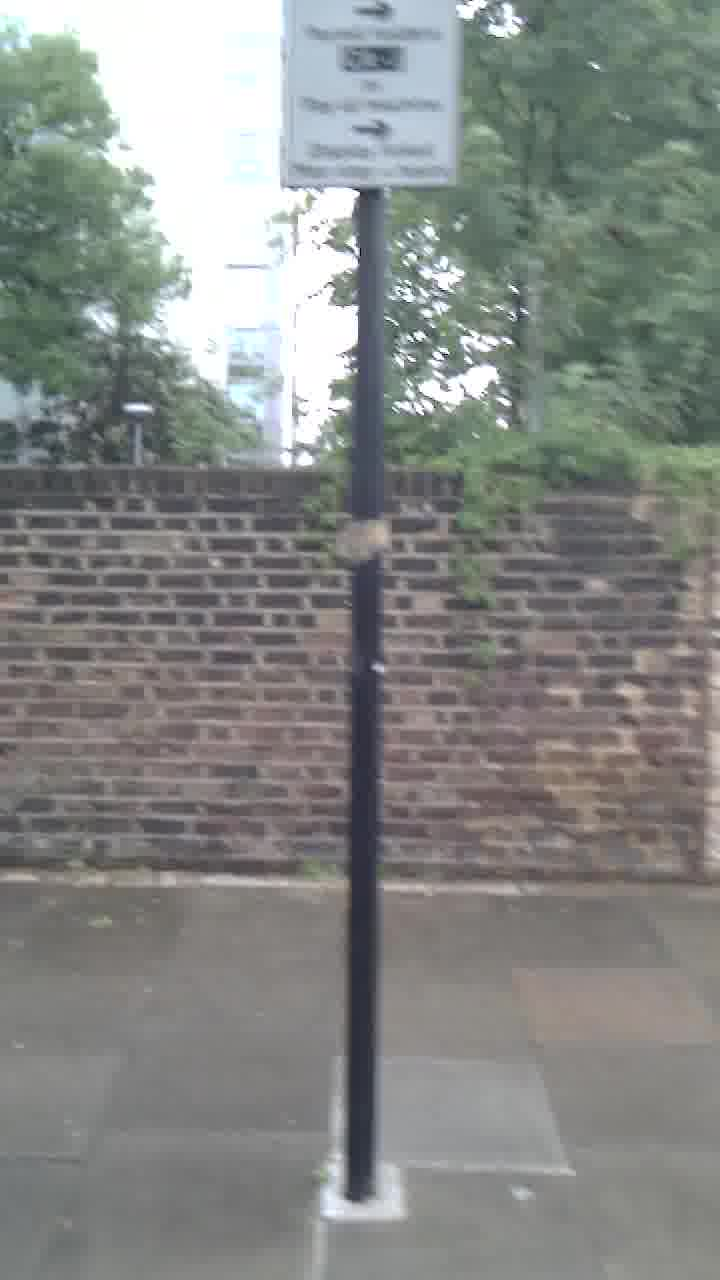
\includegraphics[width=0.3\textwidth]{img/lampposts_on_wall1_frame}  %\label{fig:}
 }
 \subfigure[Sparse point cloud and camera poses]{
  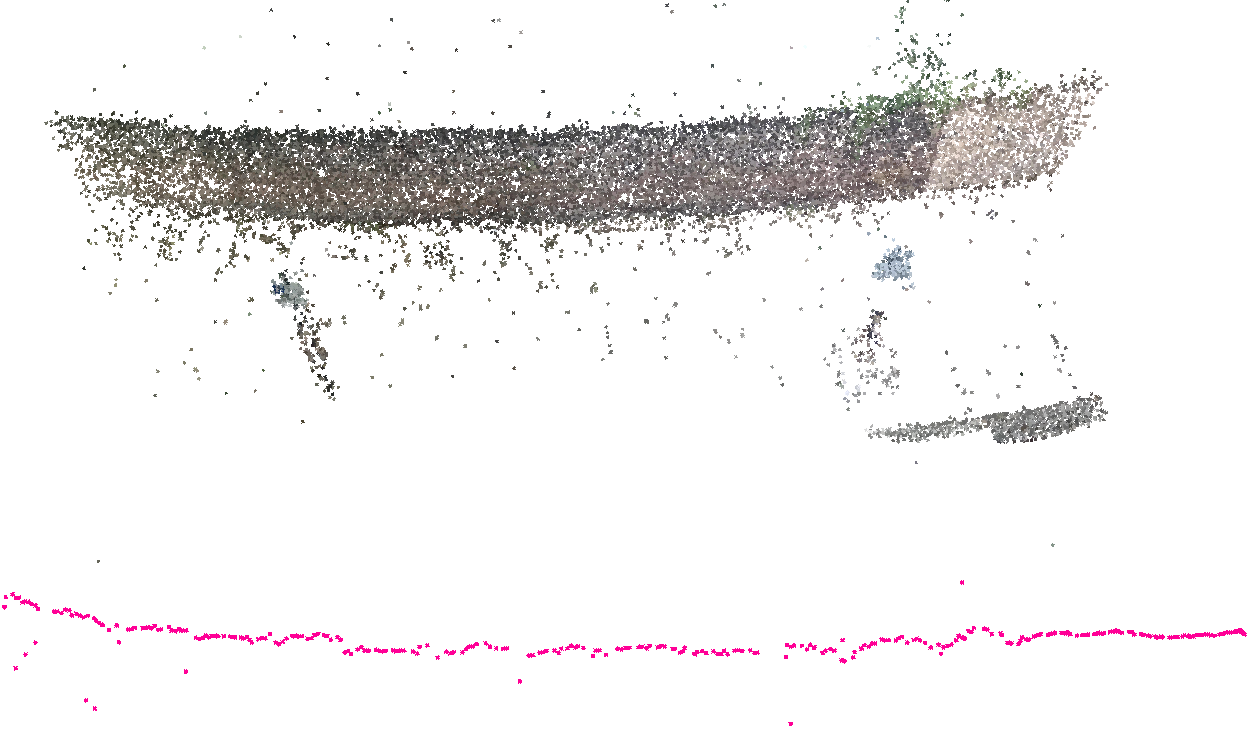
\includegraphics[width=0.65\textwidth]{img/lampposts_on_wall1_sparse}  %\label{fig:}
 }
 \subfigure[Discretised sparse point cloud ($r=1000$)]{
  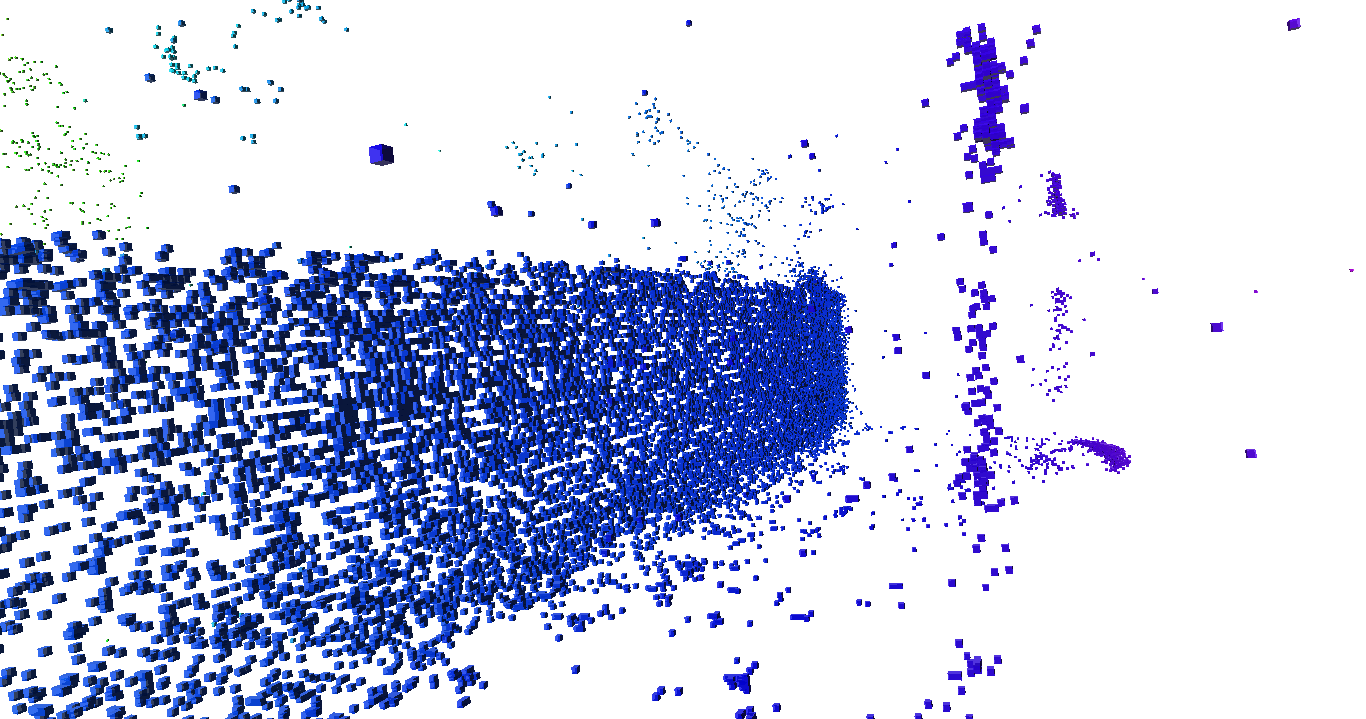
\includegraphics[width=1\textwidth]{img/lampposts_on_wall1_carve0}  %\label{fig:}
 }
 \caption{Typical result 2: lampposts\_on\_wall1 dataset}
 \label{fig:result-typical1}
\end{figure}
\begin{figure}[htb!]
 \centering
 \subfigure[Result of our Visibility Space Carving (Alg. \ref{alg:vis-carving}) with $r=500$; Notice the occupied-labelled space above and underneath the carved space, caused by an insufficient amount of feature points in the trees above the wall and on the ground.]{
  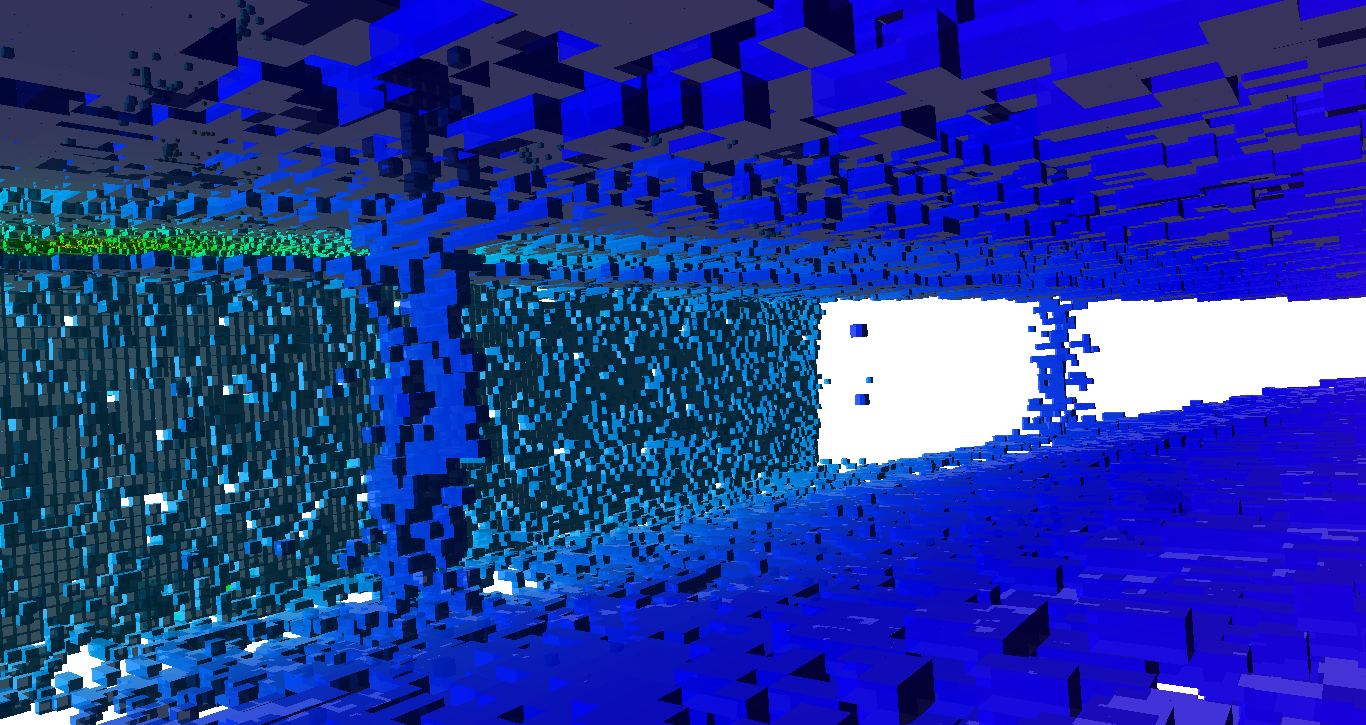
\includegraphics[width=0.95\textwidth]{img/lampposts_on_wall1_carve1}  %\label{fig:}
 }
 \subfigure[Result of our Visibility-Occlusion Space Carving Veto (Alg. \ref{alg:vis-occ-carving-veto}) with $r=1000, Pr_{incr}=0.005$]{
  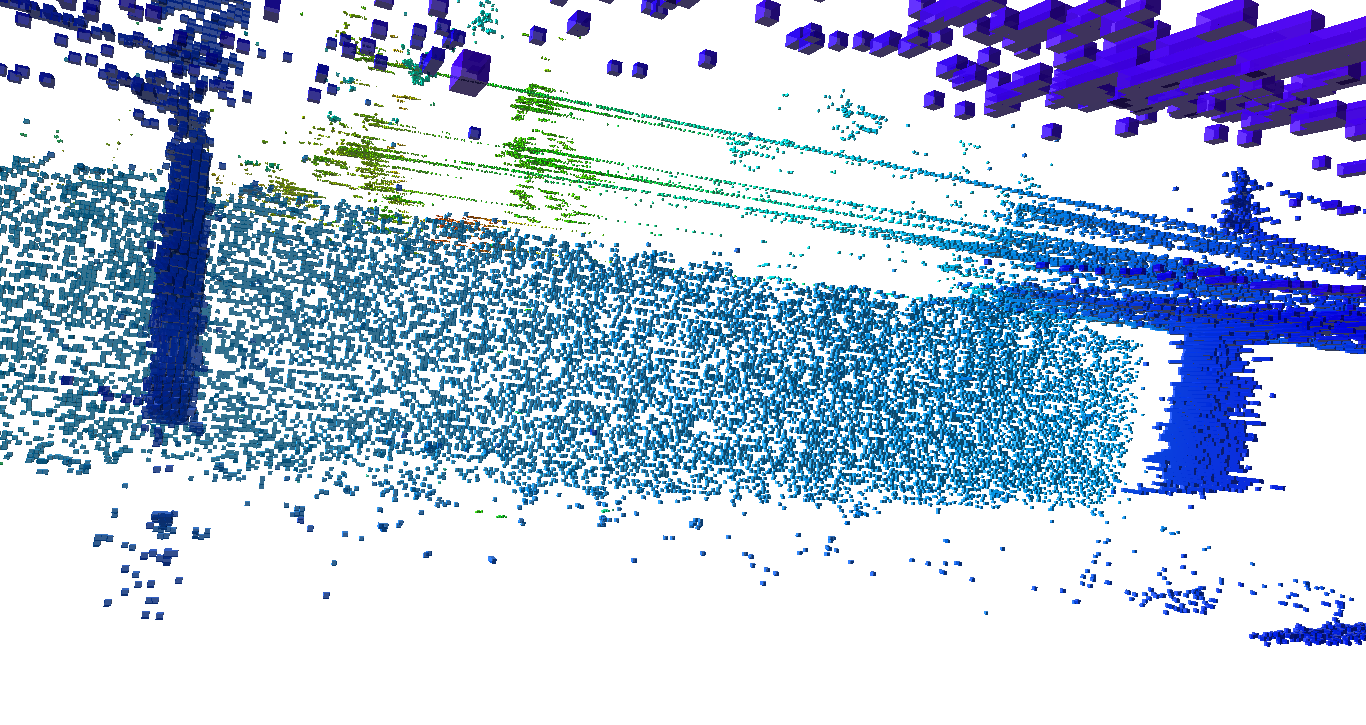
\includegraphics[width=0.95\textwidth]{img/lampposts_on_wall1_carve2}  %\label{fig:}
 }
 \subfigure[Result of CMVS/PMVS \cite{Furukawa2010}]{
  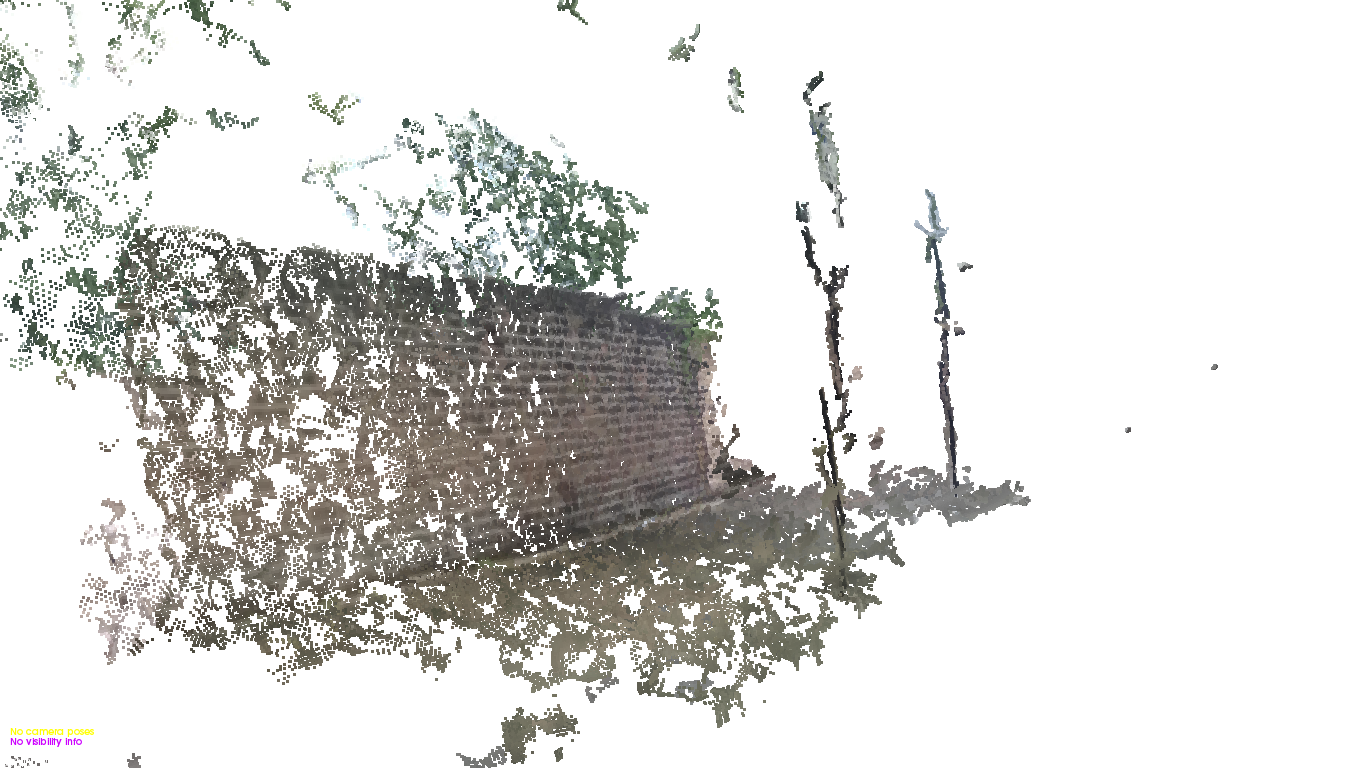
\includegraphics[width=0.95\textwidth]{img/lampposts_on_wall1_dense}  %\label{fig:}
 }
 \caption{Typical result 2: lampposts\_on\_wall1 dataset (cont.)}
 \label{fig:result-typical1-2}
\end{figure}

\begin{figure}[htb!]
 \centering
 \subfigure[Example frame]{
  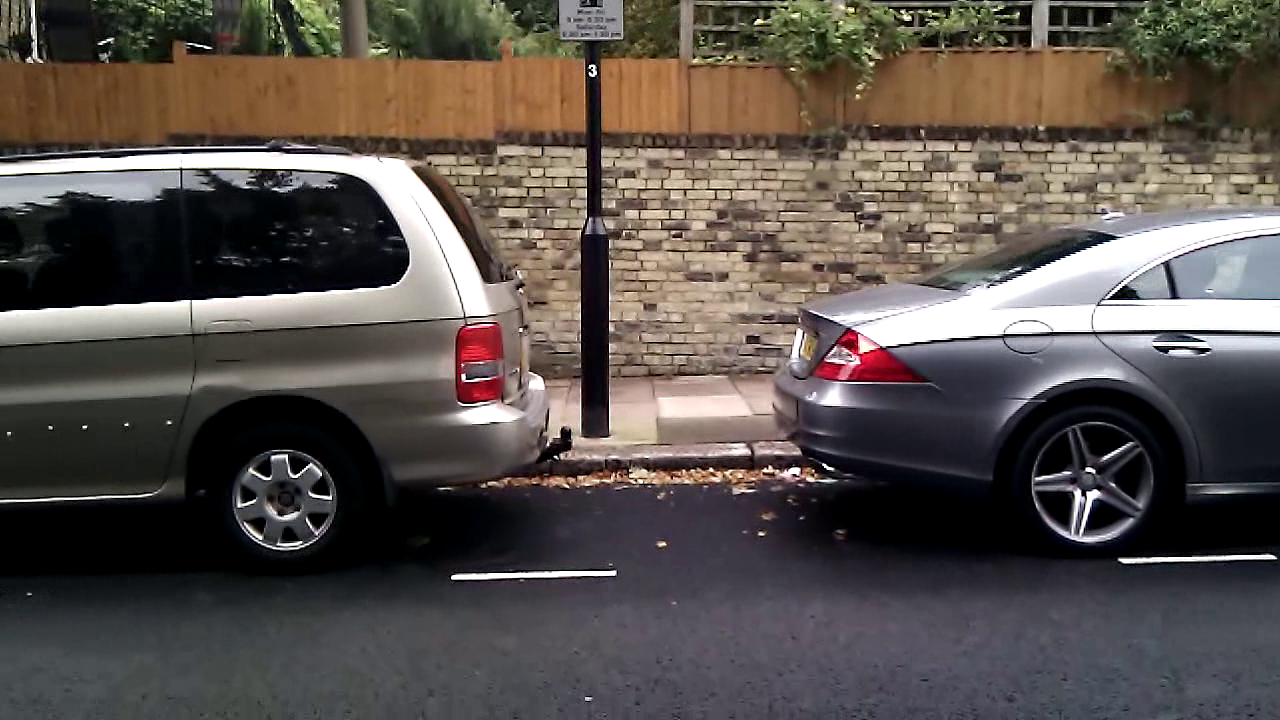
\includegraphics[width=0.9\textwidth]{img/car_and_wall1_frame}  %\label{fig:}
 }
 \subfigure[Sparse point cloud and camera poses, annotated with visibility lines from one point (hinting at possible occluding object locations)]{
  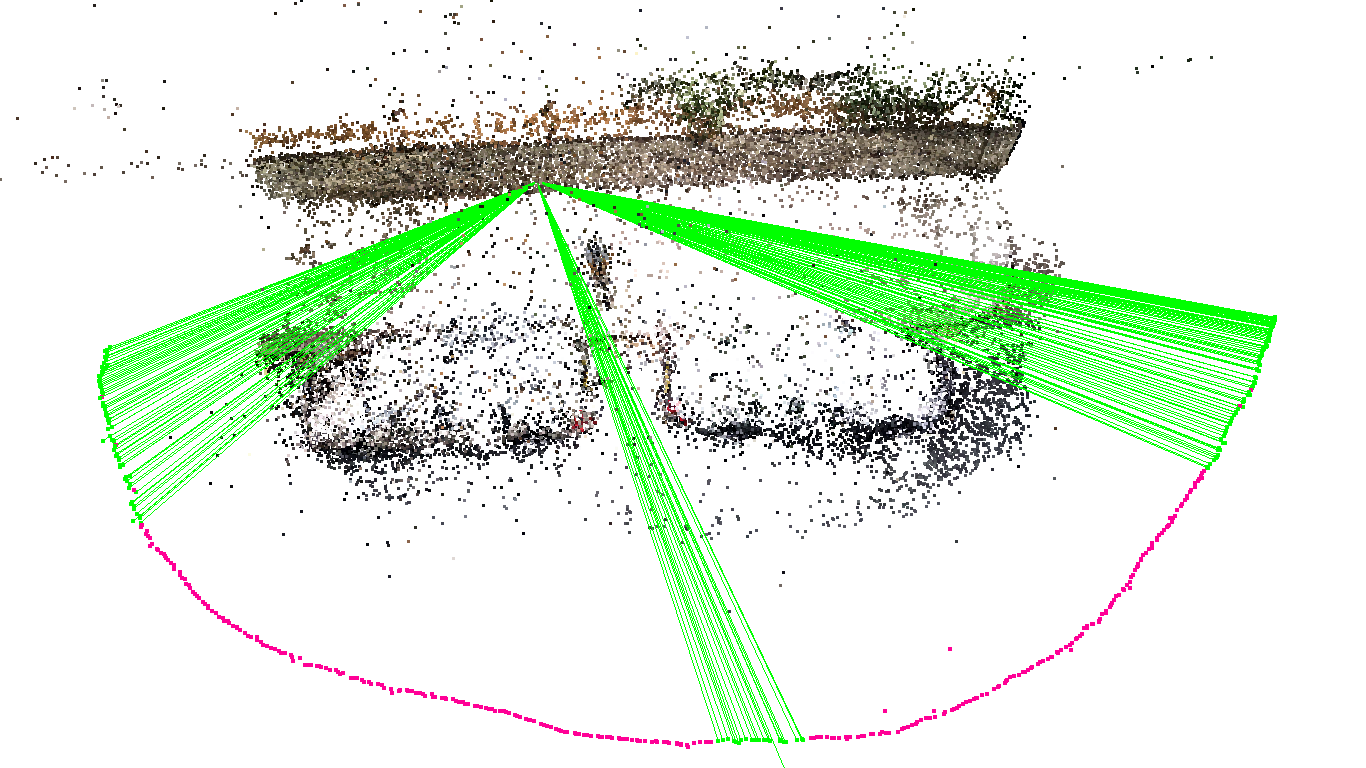
\includegraphics[width=1\textwidth]{img/car_and_wall1_sparse}  %\label{fig:}
 }
 \subfigure[Discretised sparse point cloud ($r=1000$)]{
  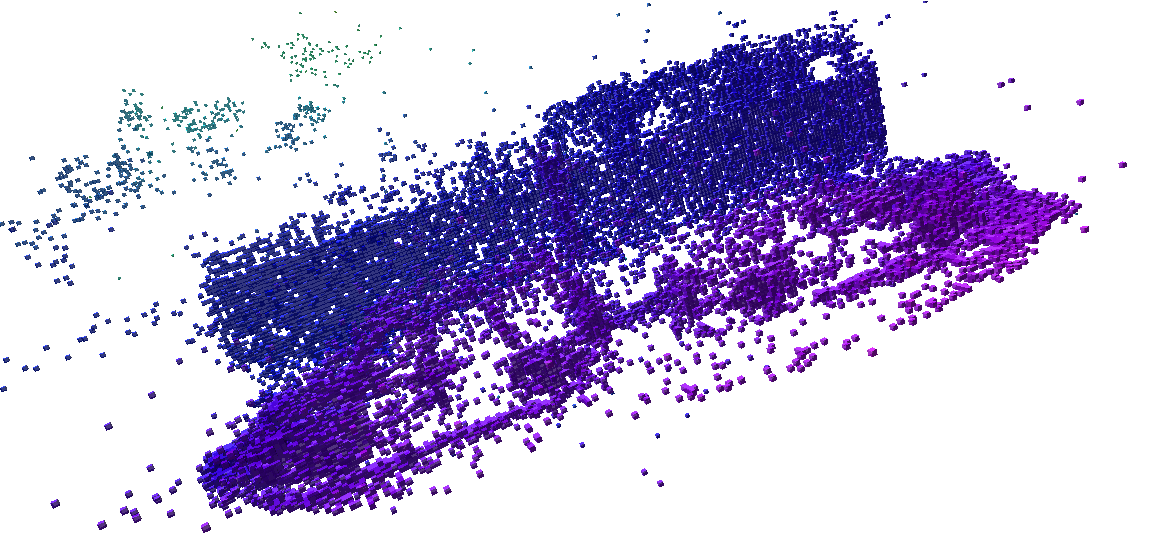
\includegraphics[width=1\textwidth]{img/car_and_wall1_carve0}  %\label{fig:}
 }
 \caption{Typical result 2: car\_and\_wall1 dataset}
 \label{fig:result-typical2}
\end{figure}
\begin{figure}[htb!]
 \centering
 \subfigure[Result of our Visibility Space Carving (Alg. \ref{alg:vis-carving}) with $r=1000$; Incorrectly occupied-labelled space inside the red `box', caused by an insuffient amount of feature points above the wall (\eg on trees), was removed for visualisation purposes.]{
  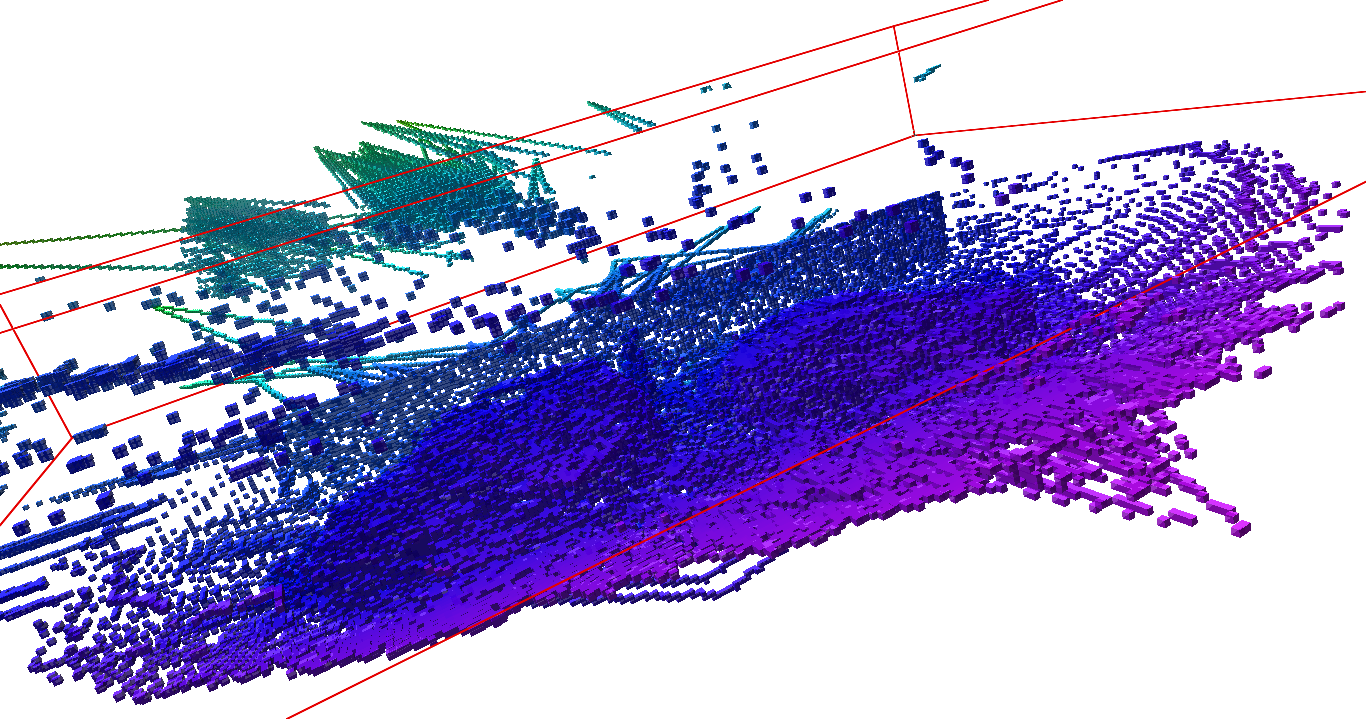
\includegraphics[width=1\textwidth]{img/car_and_wall1_carve1}  %\label{fig:}
 }
 \subfigure[Result of our Visibility-Occlusion Space Carving Veto (Alg. \ref{alg:vis-occ-carving-veto}) with $r=2500, Pr_{incr}=0.005$]{
  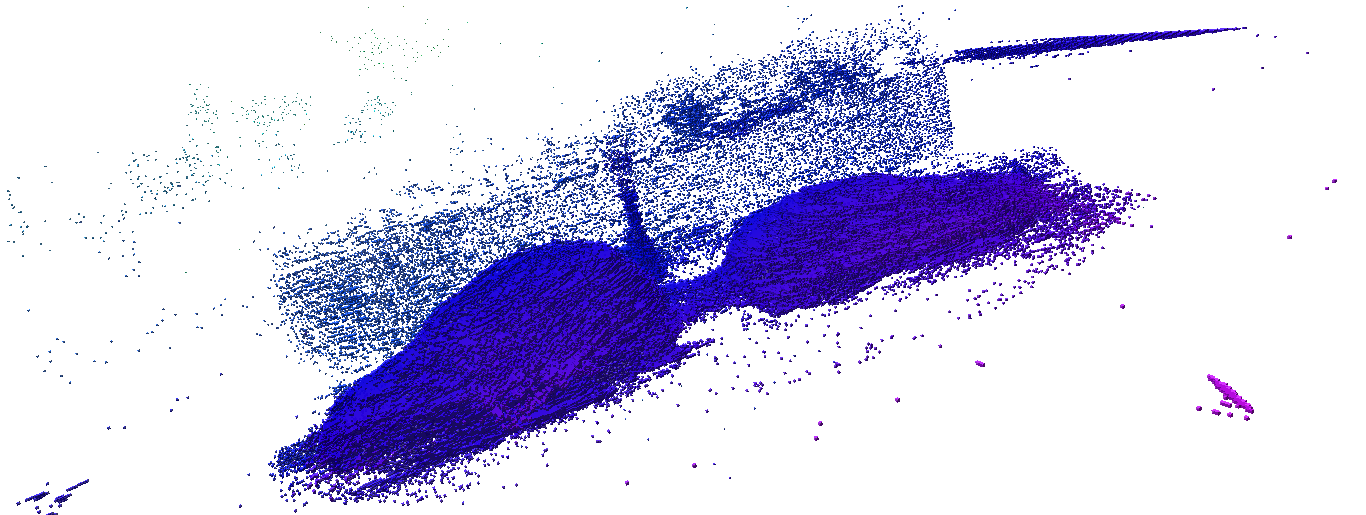
\includegraphics[width=1\textwidth]{img/car_and_wall1_carve2}  %\label{fig:}
 }
 \subfigure[Result of CMVS/PMVS \cite{Furukawa2010}]{
  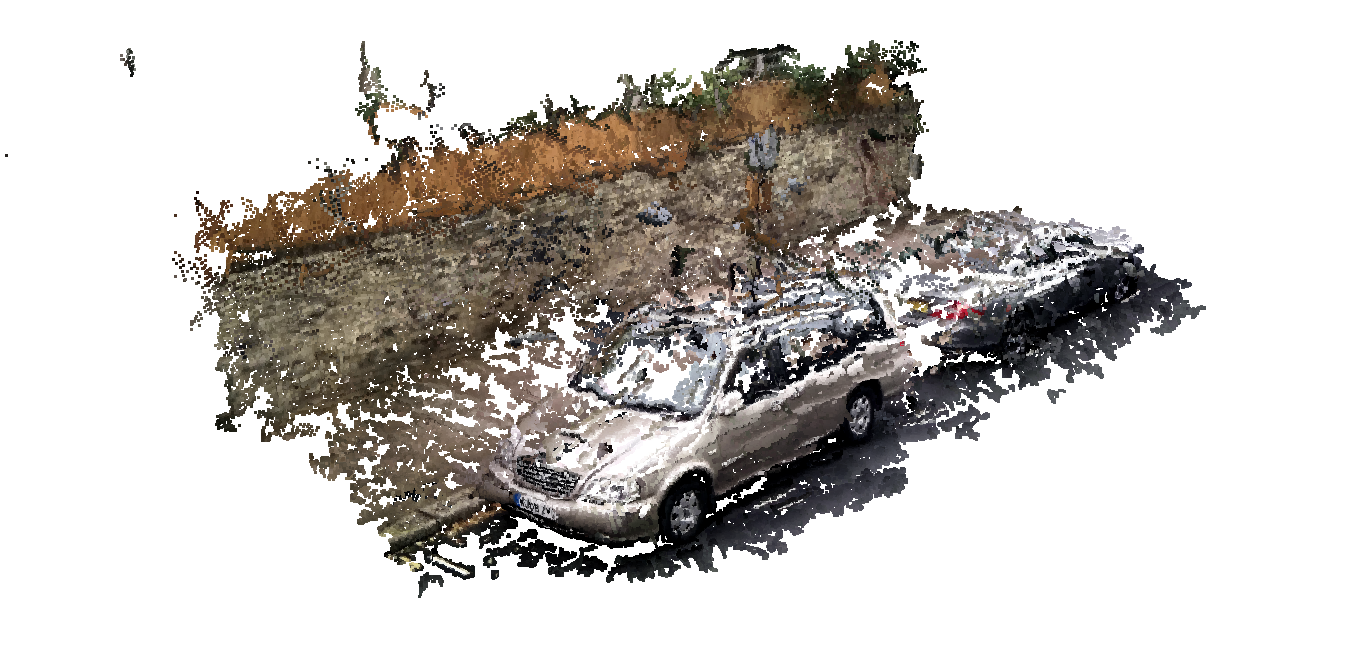
\includegraphics[width=1\textwidth]{img/car_and_wall1_dense}  %\label{fig:}
 }
 \caption{Typical result 2: car\_and\_wall1 dataset (cont.)}
 \label{fig:result-typical2-2}
\end{figure}



\begin{figure}[htb!]
 \centering
 \subfigure[Example frame]{
  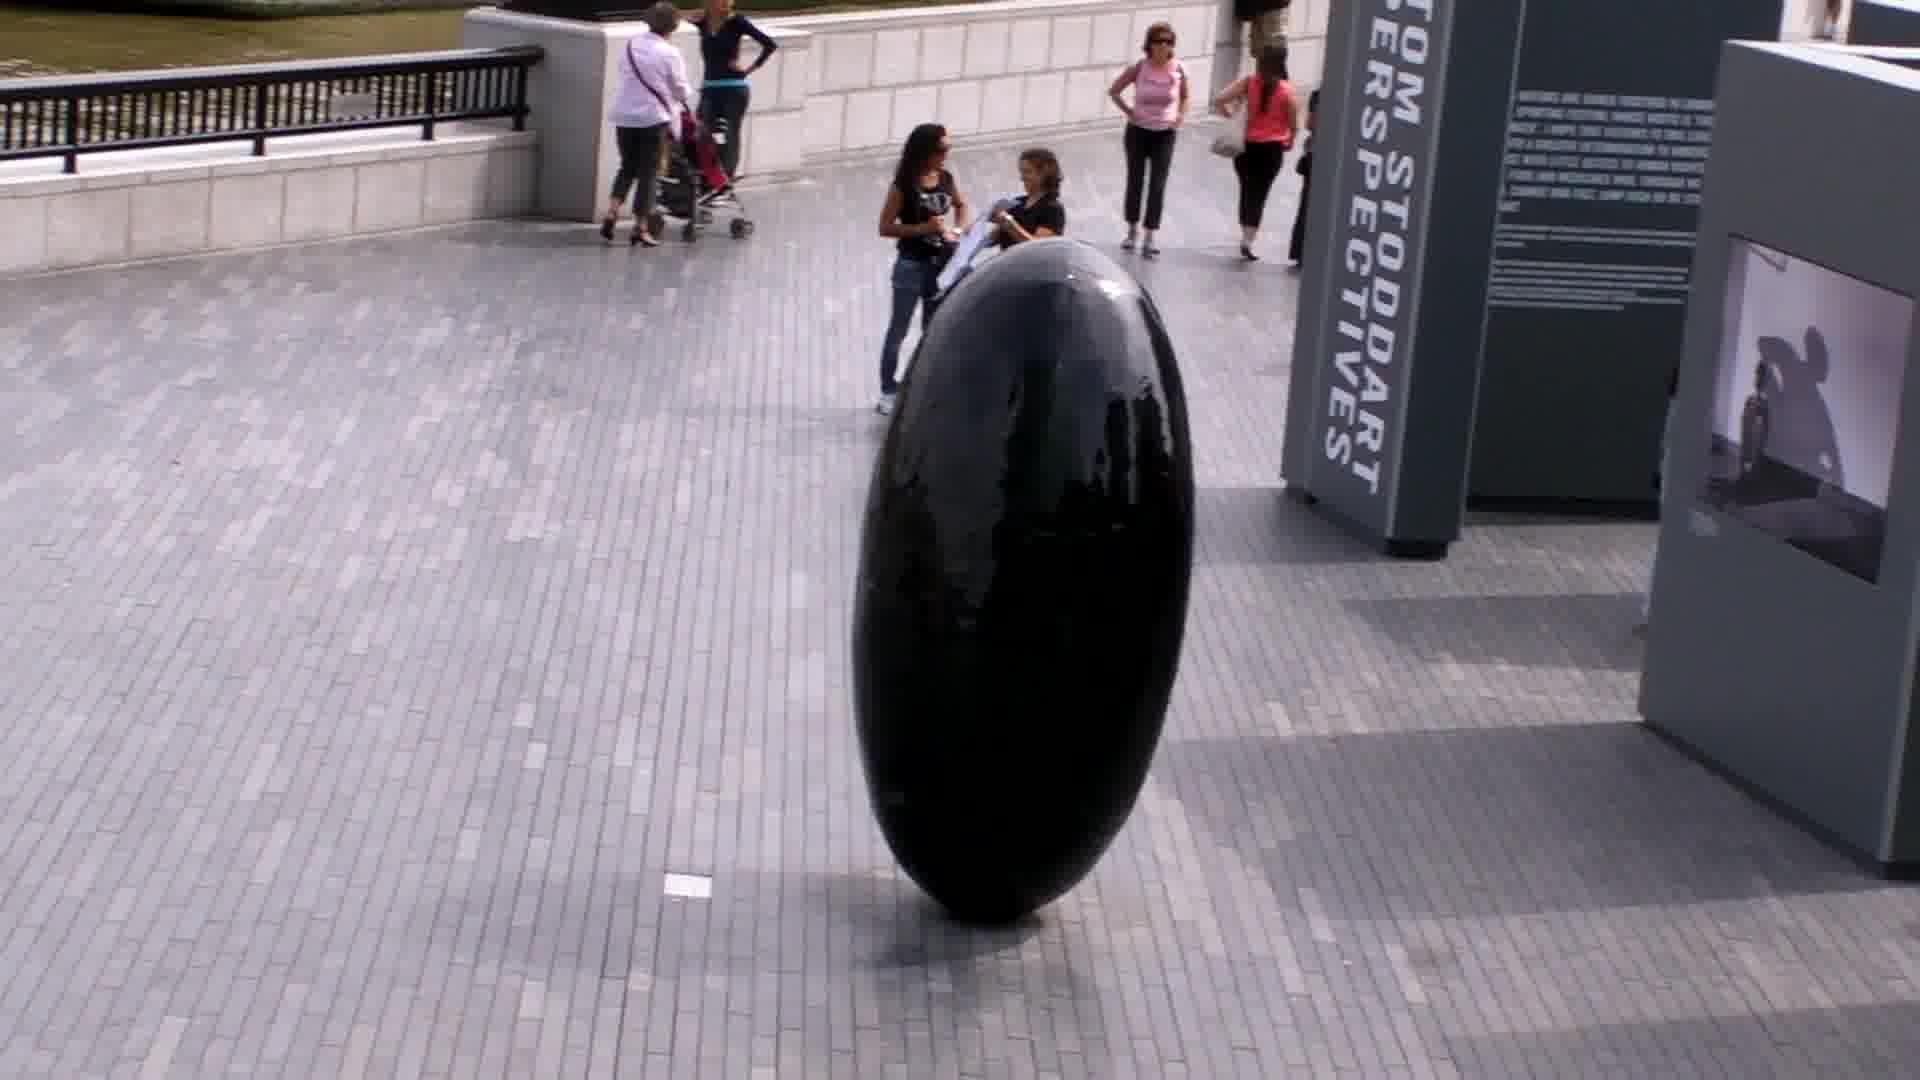
\includegraphics[width=0.9\textwidth]{img/sculpture1_frame}  %\label{fig:}
 }
 \subfigure[Sparse point cloud and camera poses, annotated with visibility lines from one point]{
  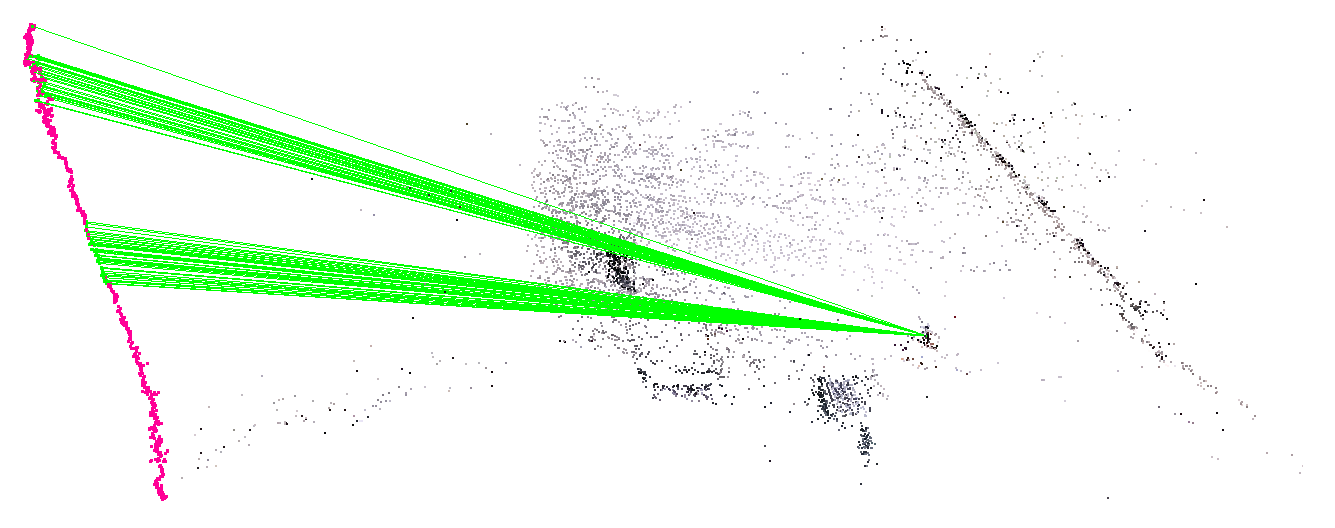
\includegraphics[width=0.9\textwidth]{img/sculpture1_sparse}  %\label{fig:}
 }
 \subfigure[Discretised sparse point cloud ($r=1000$)]{
  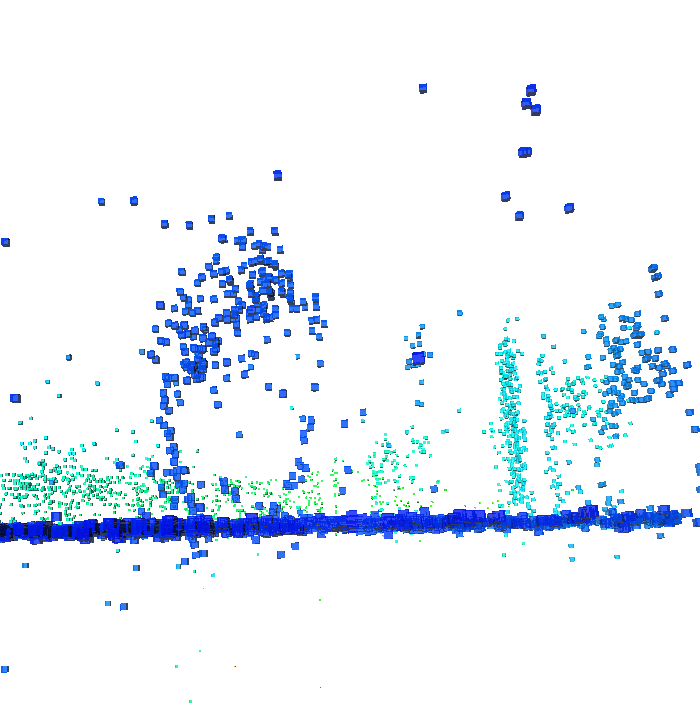
\includegraphics[width=0.45\textwidth]{img/sculpture1_carve0}  \label{fig:sculpture1_carve0}
 }
 \subfigure[Discretised sparse point cloud ($r=1000$), carveviewer; notice the incorrectly visible ground voxels (blue-ish) on the lower half of the sculpture]{
  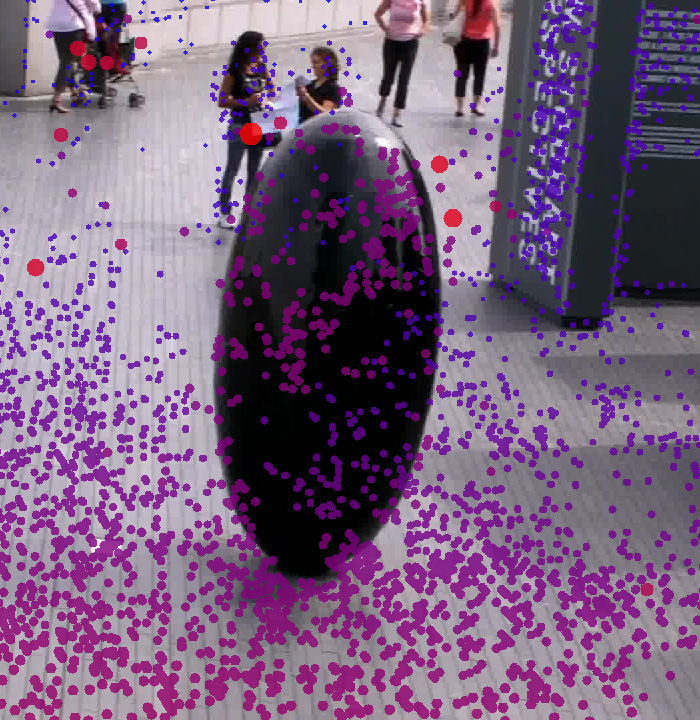
\includegraphics[width=0.45\textwidth]{img/sculpture1_carve0_ann}  %\label{fig:}
 }
 \caption{Good result 2: memorial dataset}
 \label{fig:result-good1}
\end{figure}
\begin{figure}[htb!]
 \centering
 \subfigure[Result of our Visibility Space Carving (Alg. \ref{alg:vis-carving}) with $r=250$]{
  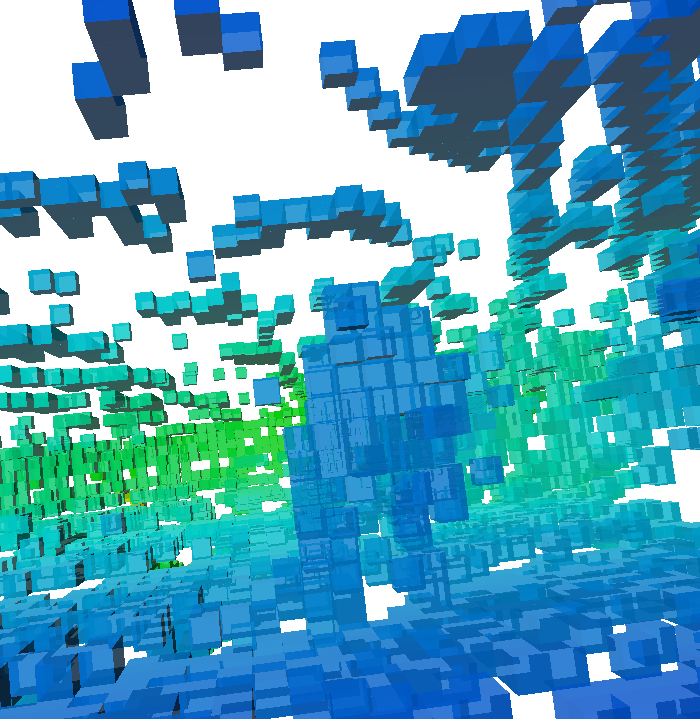
\includegraphics[width=0.45\textwidth]{img/sculpture1_carve1}  %\label{fig:}
 }
 \subfigure[Result of our Visibility Space Carving (Alg. \ref{alg:vis-carving}) with $r=250$, carveviewer]{
  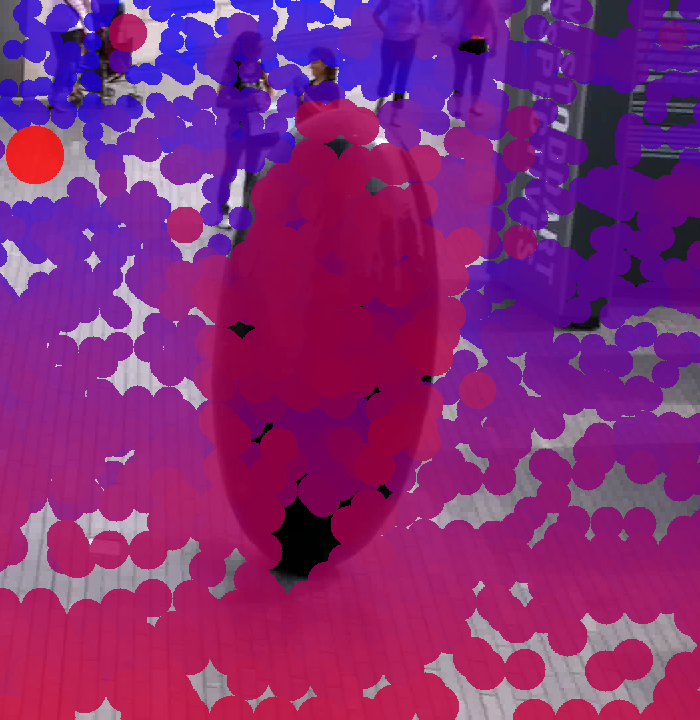
\includegraphics[width=0.45\textwidth]{img/sculpture1_carve1_ann}  %\label{fig:}
 }
 \subfigure[Result of our Visibility-Occlusion Space Carving Veto (Alg. \ref{alg:vis-occ-carving-veto}) with $r=1000, Pr_{incr}=0.001$]{
  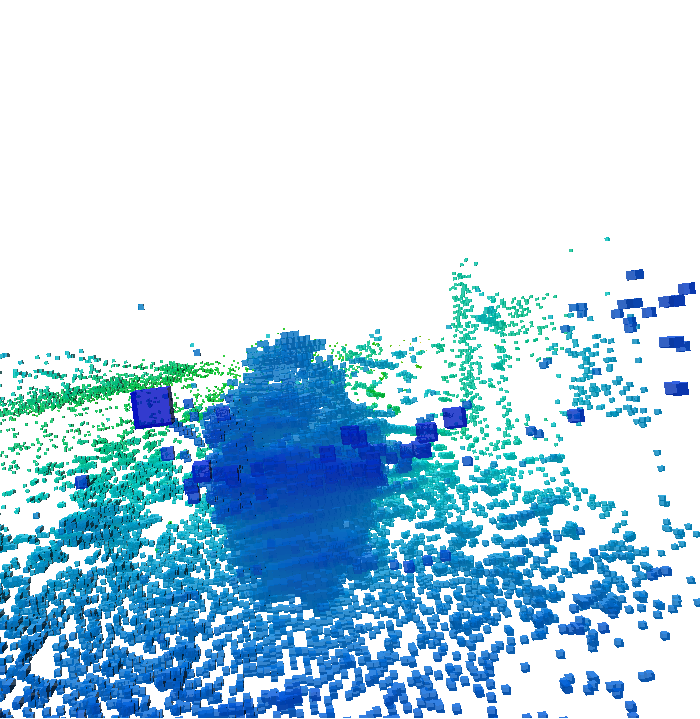
\includegraphics[width=0.45\textwidth]{img/sculpture1_carve2}  %\label{fig:}
 }
 \subfigure[Result of our Visibility-Occlusion Space Carving Veto (Alg. \ref{alg:vis-occ-carving-veto}) with $r=1000, Pr_{incr}=0.001$, carveviewer]{
  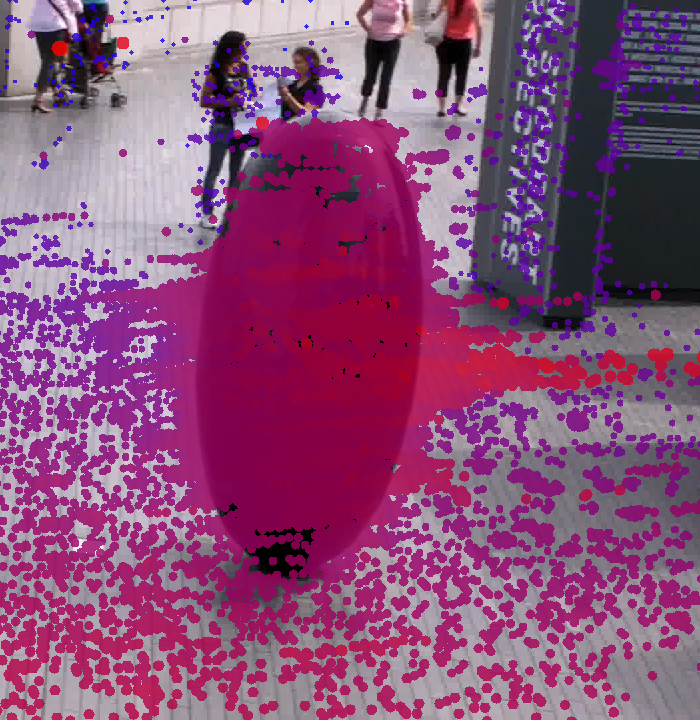
\includegraphics[width=0.45\textwidth]{img/sculpture1_carve2_ann}  %\label{fig:}
 }
 \subfigure[Result of CMVS/PMVS \cite{Furukawa2010}. Notice the similarity with the sparse point cloud as seen from this angle, shown in \ref{fig:sculpture1_carve0}; lack of texture clearly influences both sparse and dense point cloud reconstructions.]{
  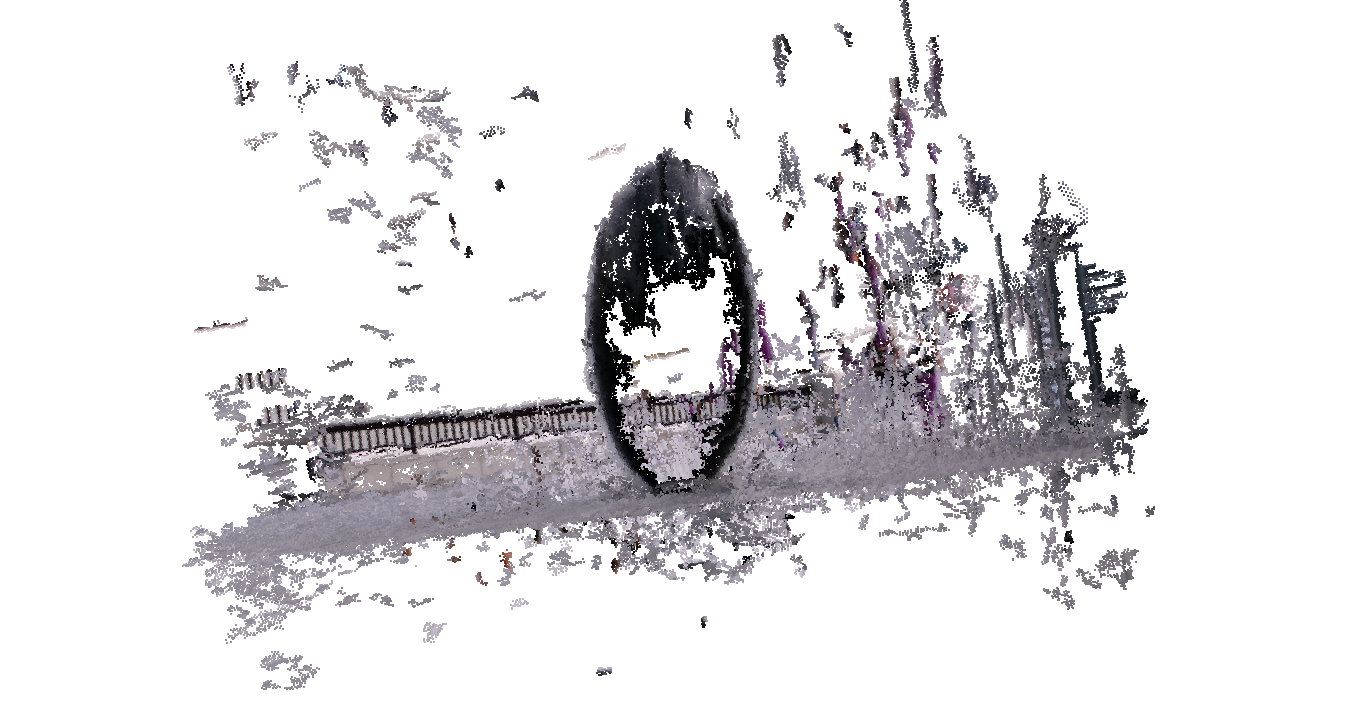
\includegraphics[width=0.90\textwidth]{img/sculpture1_dense}  %\label{fig:}
 }
 %\subfigure[Result of CMVS/PMVS \cite{Furukawa2010}, carveviewer]{
 % 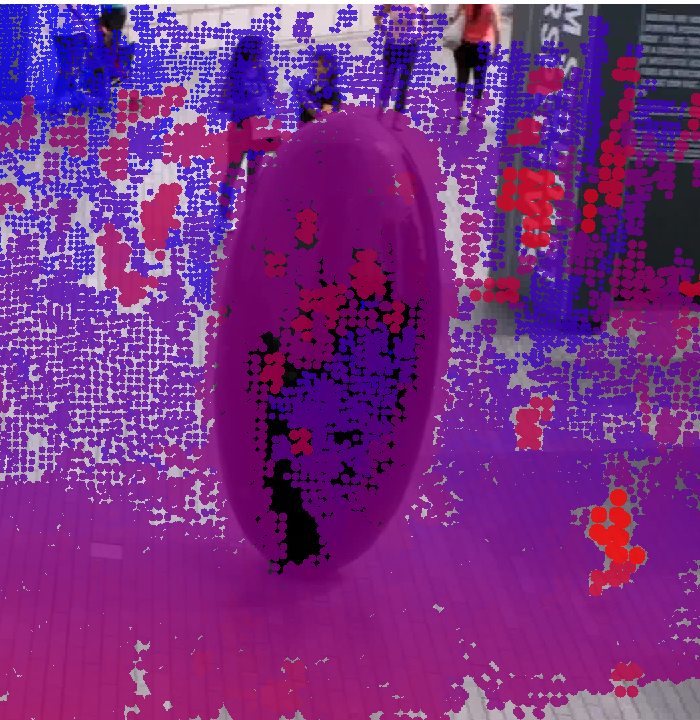
\includegraphics[width=0.45\textwidth]{img/sculpture1_dense_ann}  %\label{fig:}
 %}
 \caption{Good result 1: sculpture1 dataset (cont.)}
 \label{fig:result-good1-2}
\end{figure}


\begin{figure}[htb!]
 \centering
 \subfigure[Example frame]{
  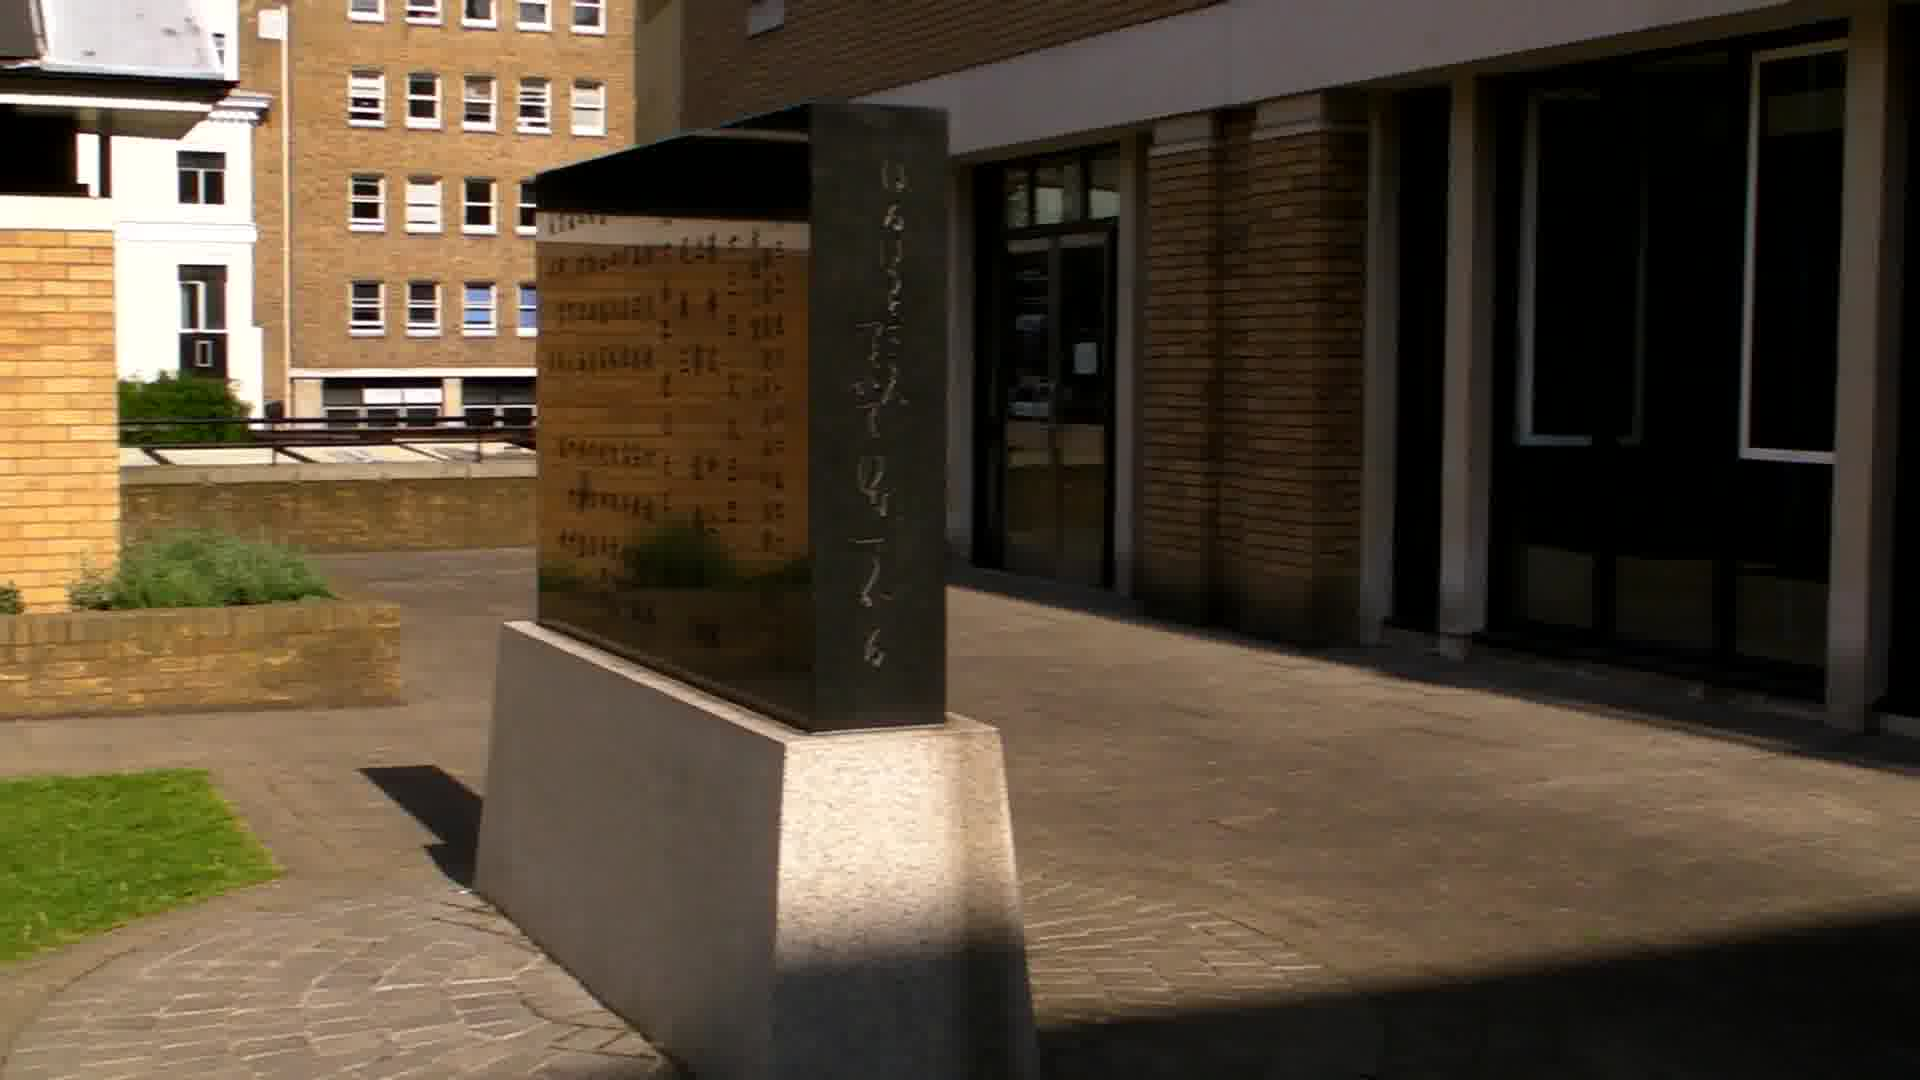
\includegraphics[width=0.9\textwidth]{img/memorial_frame}  %\label{fig:}
 }
 \subfigure[Sparse point cloud and camera poses]{
  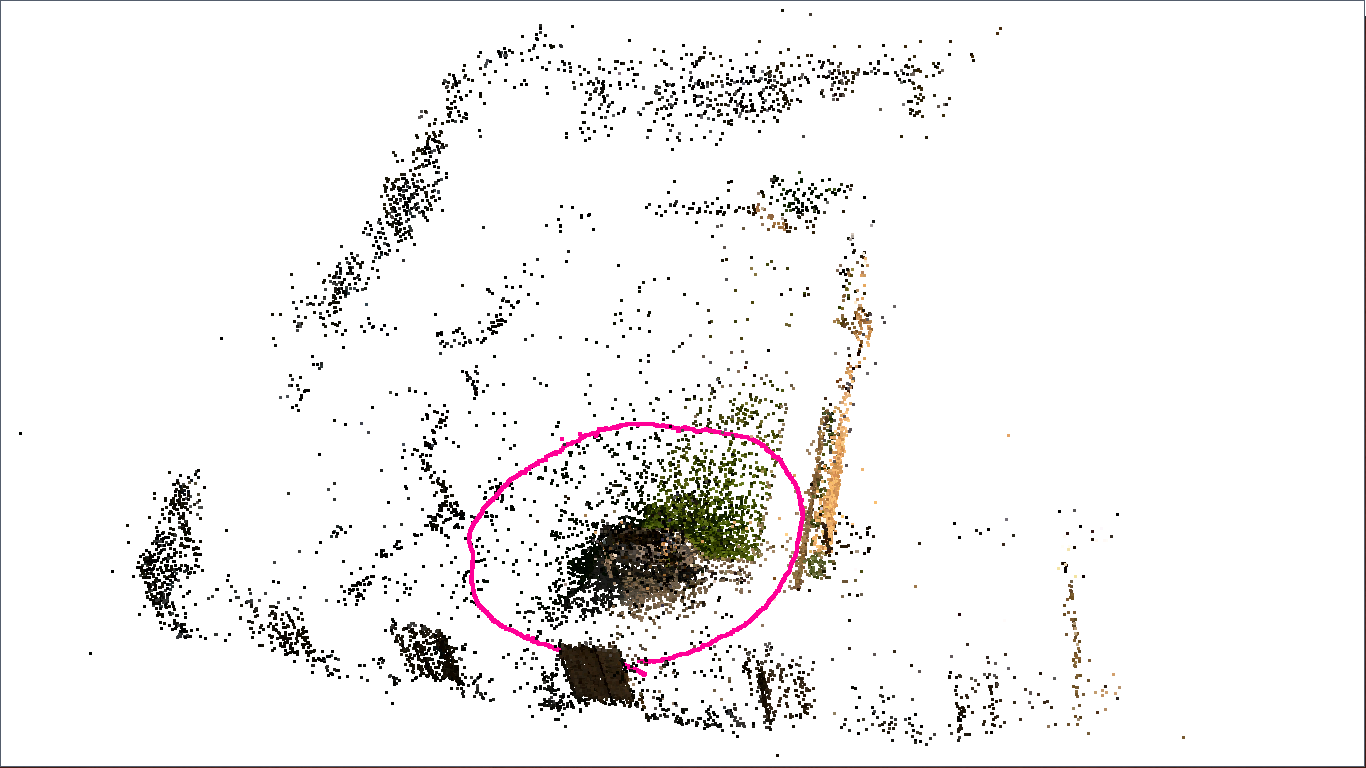
\includegraphics[width=0.9\textwidth]{img/memorial_sparse}  %\label{fig:}
 }
 \subfigure[Discretised sparse point cloud ($r=2500$)]{
  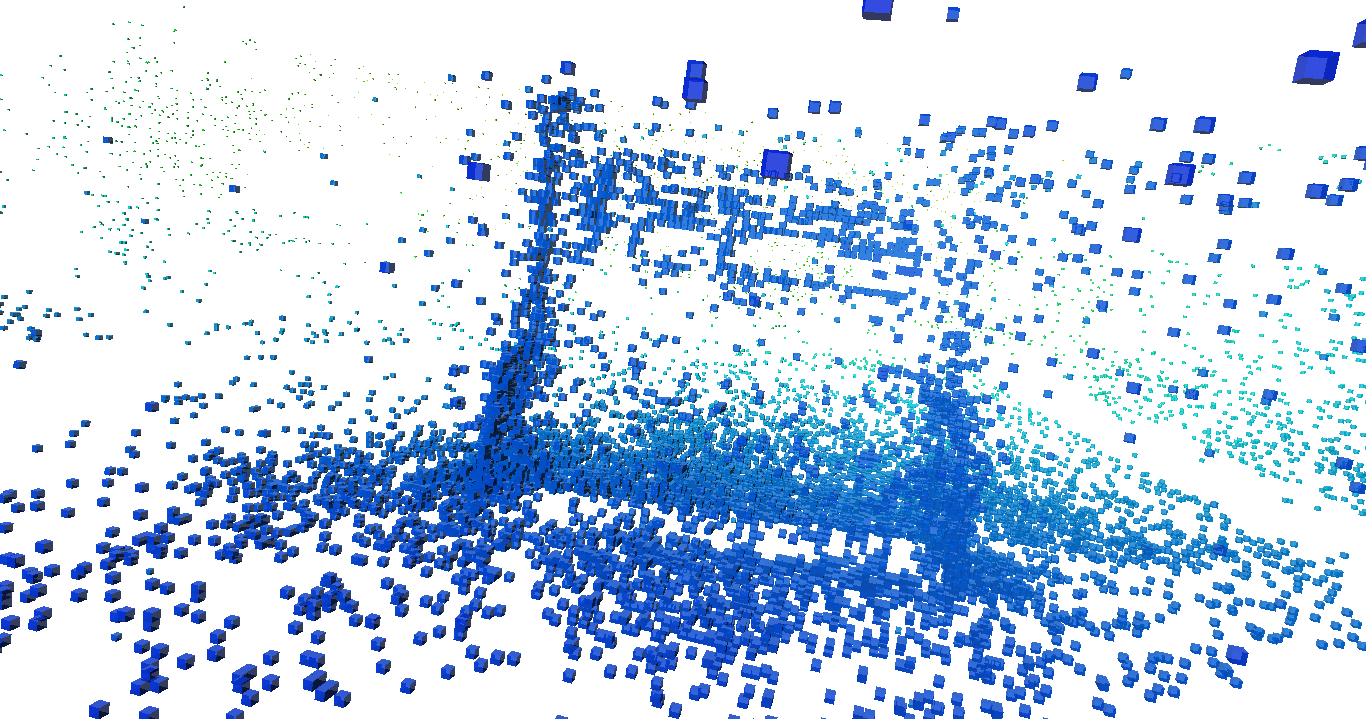
\includegraphics[width=0.9\textwidth]{img/memorial_carve0}  %\label{fig:}
 }
 \caption{Good result 2: memorial dataset}
 \label{fig:result-good2}
\end{figure}
\begin{figure}[htb!]
 \centering
 \subfigure[Result of our Visibility Space Carving (Alg. \ref{alg:vis-carving}) with $r=500$]{
  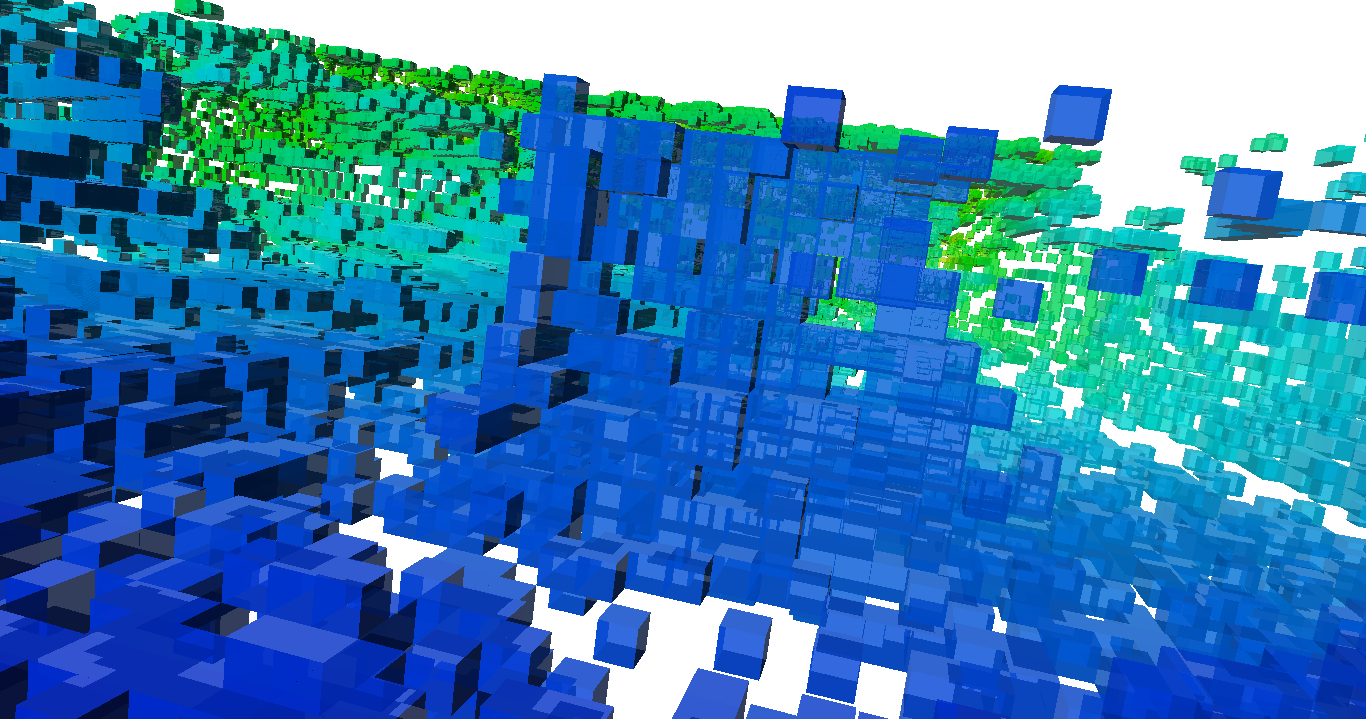
\includegraphics[width=0.9\textwidth]{img/memorial_carve1}  %\label{fig:}
 }
 \subfigure[Result of our Visibility-Occlusion Space Carving Veto (Alg. \ref{alg:vis-occ-carving-veto}) with $r=2500, Pr_{incr}=0.001$]{
  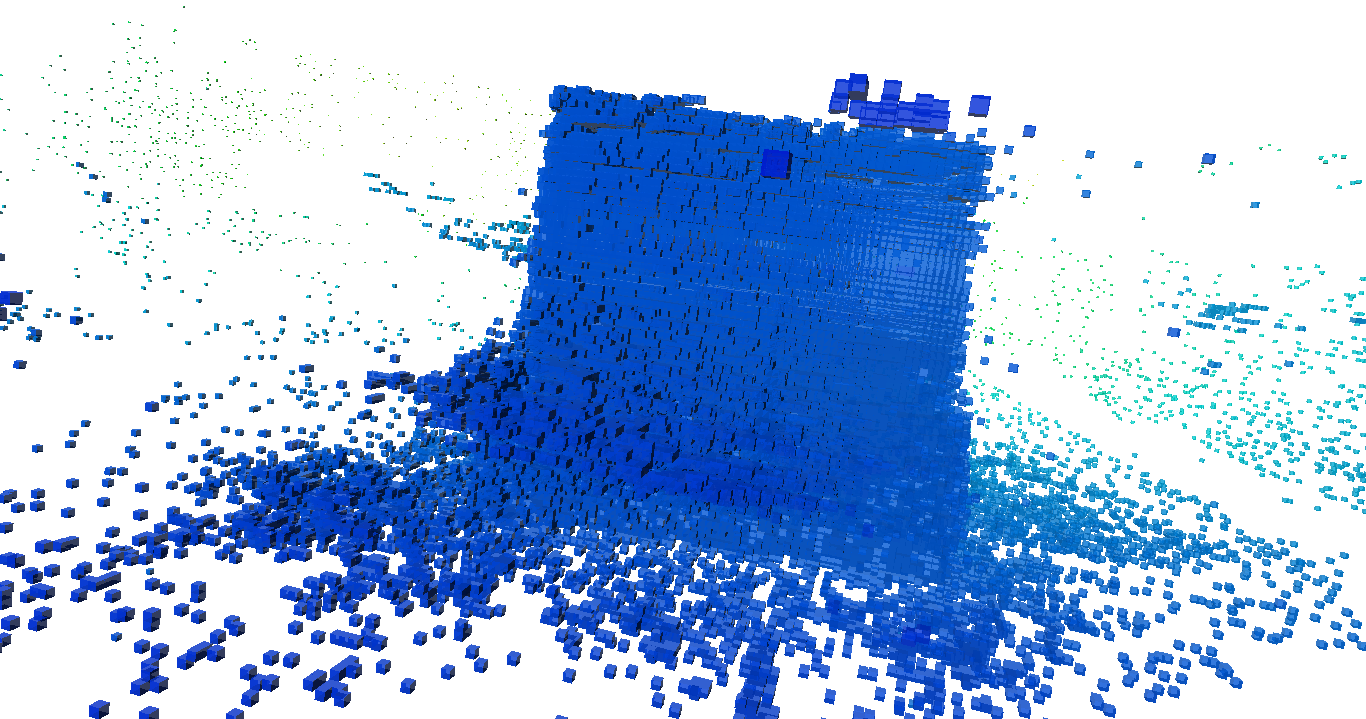
\includegraphics[width=0.9\textwidth]{img/memorial_carve2}  %\label{fig:}
 }
 \subfigure[Result of CMVS/PMVS \cite{Furukawa2010}]{
  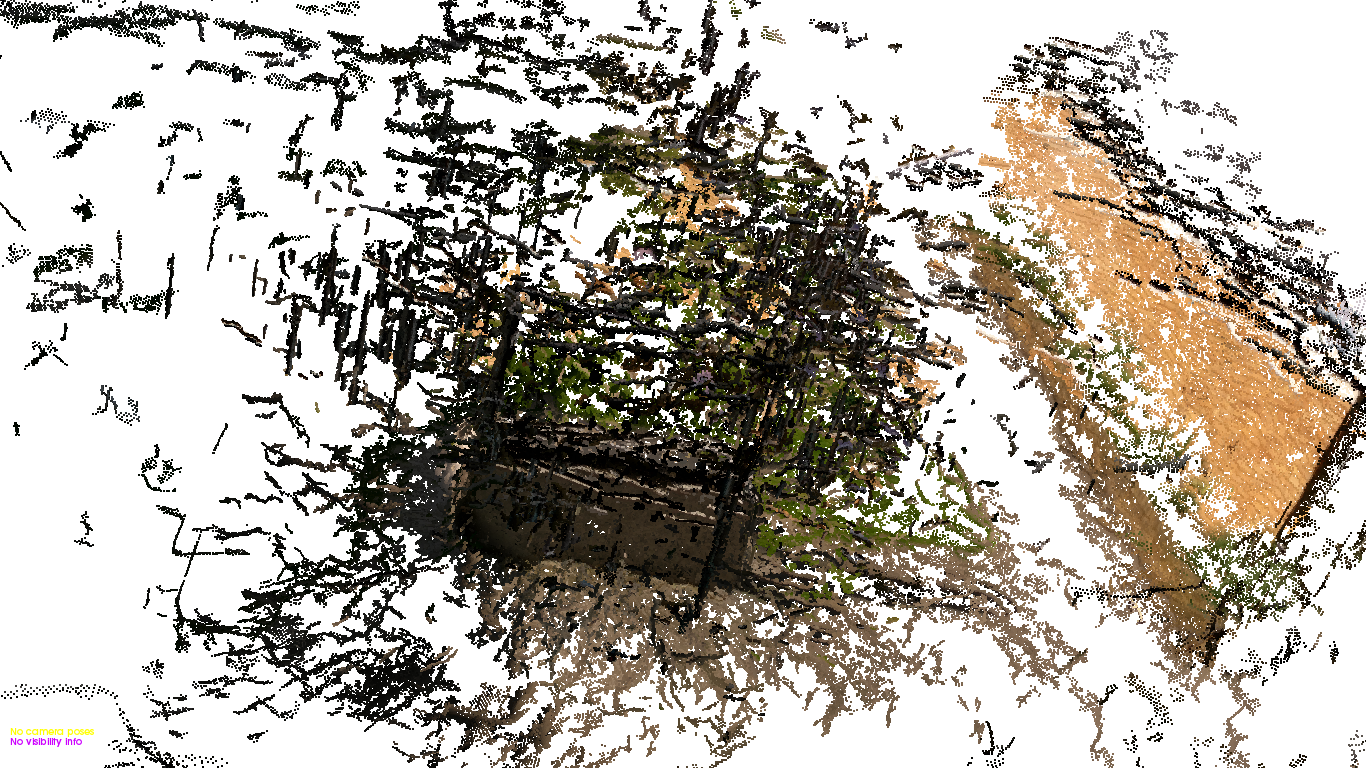
\includegraphics[width=0.9\textwidth]{img/memorial_dense}  %\label{fig:}
 }
 \caption{Good result 2: memorial dataset (cont.)}
 \label{fig:result-good2-2}
\end{figure}


% TODO: results regularisation
% TODO: results carve3
% TODO: results photofly



%% Evaluation
\section{Evaluation}
% describe results

%- write about all four
%  - 1: poor img quality, only parallel movement; mostly carved where wall was behind
%  - 2: 
%
%- comparable for small low-textured
%- dense misses parts of bigger low-textured objects
%- ours better for reflective objects: state-of-the-art dense reconstruction gives lots of junk/mess/huddle in the air due to wrong triangulation (which is only visible in dense due to lower confidence necessary)
%- quality of the camera not that important
%
%
%% discussion + limitations (data, features, parameters)
%- low-textured obj (pilars etc) and reflective buildings surprisingly often in urban (outdoor) environments
%- promising method, however:
%  - needs enough texture (lots of data can help); will get occupied space if within occlusion rays and not proven otherwise
%  - unstable features cause problems
%  - since carving tubes, max resolution (thus finding bigger green screens -> future research section), and r dependent on amount of data

